% SpatialMoE-SOD routing mechanism (Fig. 2)
%
% Companion to fig_architecture.tex and deliberately sharing its design tokens
% (same palette, same 6 pt `base` font, same box / arrow styles), so the two
% figures read as a set. The flow is vertical here because the point of the
% figure is the branch: the entropy is taken from the *logits*, over all eight
% experts, not from the top-2 selection.
%
% Canvas is 104 mm wide, so include it at about 0.68\textwidth; every label then
% prints at its true 6 pt size. No thumbnails, so nothing here depends on ./figs.
\documentclass[tikz,border=0pt]{standalone}
\usepackage[T1]{fontenc}
\usepackage{helvet}
\renewcommand{\familydefault}{\sfdefault}
\usepackage{amsmath,amssymb}
\usepackage{sansmath}
\usetikzlibrary{arrows.meta,calc}

% ---------------------------------------------------------------- palette (same as Fig. 1)
\definecolor{bbF}{HTML}{DCE8F5}  \definecolor{bbS}{HTML}{4F76A3}
\definecolor{moF}{HTML}{FBEFC2}  \definecolor{moS}{HTML}{B08D2B}  \definecolor{moD}{HTML}{E9CF74}
\definecolor{enF}{HTML}{F8DCC8}  \definecolor{enS}{HTML}{C07A3E}
\definecolor{dcF}{HTML}{DCEBD2}  \definecolor{dcS}{HTML}{6B8F4E}
\definecolor{hdF}{HTML}{E4DDF0}  \definecolor{hdS}{HTML}{7D6AA3}
\definecolor{ink}{HTML}{333333}  \definecolor{sup}{HTML}{777777}

\tikzset{
  base/.style={font=\sansmath\sffamily\fontsize{6}{7}\selectfont, align=center, text=black},
  box/.style={base, draw, line width=0.5pt, rounded corners=1.5pt, inner sep=1.5pt},
  flow/.style={-{Stealth[length=1.5mm,width=1.2mm]}, line width=0.6pt, draw=ink, rounded corners=2pt},
  conf/.style={flow, draw=enS, dash pattern=on 2pt off 1.5pt},
  plus/.style={draw=enS, fill=enF, line width=0.5pt},
}

\begin{document}
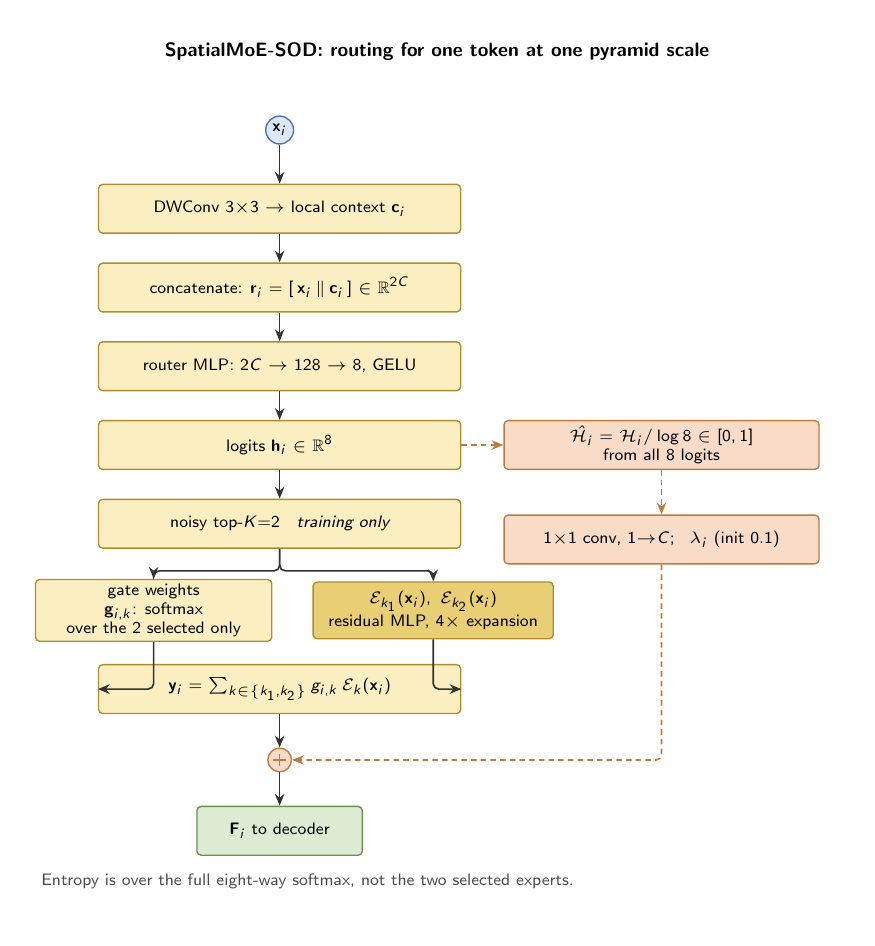
\begin{tikzpicture}[x=1cm,y=1cm]
\useasboundingbox (0,-0.05) rectangle (10.4,11.25);

% ------------------------------------------------------------------ title
\node[font=\sansmath\sffamily\fontsize{7}{8}\selectfont\bfseries] at (5.2,10.95)
  {SpatialMoE-SOD: routing for one token at one pyramid scale};

% ------------------------------------------------------------------ router spine
\node[circle, draw=bbS, fill=bbF, line width=0.5pt, inner sep=1.2pt,
      font=\sansmath\sffamily\fontsize{6}{7}\selectfont] (x) at (3.2,9.95) {$\mathbf{x}_i$};
\node[box, draw=moS, fill=moF, minimum width=4.6cm, minimum height=0.62cm] (dw) at (3.2,8.95)
  {DWConv $3{\times}3$ $\to$ local context $\mathbf{c}_i$};
\node[box, draw=moS, fill=moF, minimum width=4.6cm, minimum height=0.62cm] (cat) at (3.2,7.95)
  {concatenate: $\mathbf{r}_i=[\,\mathbf{x}_i\,\|\,\mathbf{c}_i\,]\in\mathbb{R}^{2C}$};
\node[box, draw=moS, fill=moF, minimum width=4.6cm, minimum height=0.62cm] (mlp) at (3.2,6.95)
  {router MLP: $2C\to128\to 8$, GELU};
\node[box, draw=moS, fill=moF, minimum width=4.6cm, minimum height=0.62cm] (h) at (3.2,5.95)
  {logits $\mathbf{h}_i\in\mathbb{R}^{8}$};
\node[box, draw=moS, fill=moF, minimum width=4.6cm, minimum height=0.62cm] (topk) at (3.2,4.95)
  {noisy top-$K{=}2$ \; {\itshape training only}};

% ------------------------------------------------------------------ branch: gates and experts
\node[box, draw=moS, fill=moF, minimum width=3.0cm, minimum height=0.72cm] (gate) at (1.6,3.85)
  {gate weights\\$\mathbf{g}_{i,k}$: softmax\\over the 2 selected only};
\node[box, draw=moS, fill=moD, minimum width=3.05cm, minimum height=0.72cm] (exp) at (5.15,3.85)
  {$\mathcal{E}_{k_1}(\mathbf{x}_i),\;\mathcal{E}_{k_2}(\mathbf{x}_i)$\\residual MLP, $4\times$ expansion};

\node[box, draw=moS, fill=moF, minimum width=4.6cm, minimum height=0.62cm] (sum) at (3.2,2.85)
  {$\mathbf{y}_i=\sum_{k\in\{k_1,k_2\}} g_{i,k}\,\mathcal{E}_k(\mathbf{x}_i)$};

% ------------------------------------------------------------------ entropy chain (from the logits)
\node[box, draw=enS, fill=enF, minimum width=4.0cm, minimum height=0.62cm] (ent) at (8.05,5.95)
  {$\hat{\mathcal{H}}_i=\mathcal{H}_i/\log 8\in[0,1]$\\from all 8 logits};
\node[box, draw=enS, fill=enF, minimum width=4.0cm, minimum height=0.62cm] (conv) at (8.05,4.75)
  {$1{\times}1$ conv, $1{\to}C$; \, $\lambda_i$ (init $0.1$)};

\node[circle, plus, inner sep=0, minimum size=0.3cm] (P) at (3.2,1.95) {};
\draw[enS, line width=0.5pt] (3.2-0.08,1.95) -- (3.2+0.08,1.95) (3.2,1.95-0.08) -- (3.2,1.95+0.08);
\node[box, draw=dcS, fill=dcF, minimum width=2.1cm, minimum height=0.62cm] (F) at (3.2,1.05)
  {$\mathbf{F}_i$ to decoder};

% ------------------------------------------------------------------ arrows
\draw[flow] (x) -- (dw);
\draw[flow] (dw) -- (cat);
\draw[flow] (cat) -- (mlp);
\draw[flow] (mlp) -- (h);
\draw[flow] (h) -- (topk);
\draw[flow] (topk.south) -- ++(0,-0.28) -| (gate.north);
\draw[flow] (topk.south) -- ++(0,-0.28) -| (exp.north);
\draw[flow] (gate.south) |- (sum.west);
\draw[flow] (exp.south)  |- (sum.east);
\draw[flow] (sum.south) -- (P.north);
\draw[flow] (P.south) -- (F.north);
% the entropy path leaves the LOGITS, not the top-2 output
\draw[conf] (h.east) -- (ent.west);
\draw[conf] (ent.south) -- (conv.north);
\draw[conf] (conv.south) -- (8.05,1.95) -- (P.east);

% ------------------------------------------------------------------ annotation
\node[base, anchor=north west, text=black!70] at (0.05,0.62)
  {Entropy is over the full eight-way softmax, not the two selected experts.};

\end{tikzpicture}
\end{document}
